\documentclass{article}
%for the accent
\usepackage[utf8]{inputenc}
%to put an image
\usepackage{graphicx}
\usepackage[french]{babel}
\usepackage[]{amsmath, amsfonts, amssymb, enumerate}
\usepackage{pdfpages} 
\usepackage[linkbordercolor=white]{hyperref}
\selectlanguage{french}
\usepackage[utf8]{inputenc}
%all the things to make a good title
\title{PROJET GENIE LOGICIEL (SINFO015) :\\ Rapport de développement}
\author{\textbf{Auteurs}: \\ Adrien Fievet \\ Claire D'Haene \\ Julien Ladeuze \\ Maxime Dupuis}
\date{2022-2023}

\begin{document}

\maketitle

%to skip lines
\vspace{7\baselineskip}

\begin{minipage}{0.4\textwidth}
	\begin{flushleft}
		\large
		\textit{Titulaire}\\
		Tom \textsc{Mens}\\
		\textit{Enseignants}\\
		Sébastien \textsc{Bonte}\\
		Jeremy \textsc{Dubrulle}\\
		Pierre \textsc{Hauweele}	
	\end{flushleft}
\end{minipage}
~
\begin{minipage}{0.5\textwidth}
	\begin{flushright}
		\large
		\textit{Equipe 7}\\
		Adrien (220625) 4\\
		Claire (220323) 1\\
		Julien (220101) 10\\
		Maxime (212107) 7\\
	\end{flushright}
\end{minipage}

%insert the image
\begin{figure}
    \centering
    
\includegraphics[width = 0.3\textwidth]{images/umons.jpeg}
    \hspace{5em}
    
\includegraphics[width = 0.3\textwidth]{images/facSciences.png}
\end{figure}

%hide the number of the actual page just for the cover page
\thispagestyle{empty}

\newpage
\tableofcontents
\newpage

\section{Introduction: 1.6.4: Analyse statistique de la consommation énergétique}

\begin{flushleft}
Le but de cette extension est surtout de permettre au client de comparer ces données de consommation avec d'autres. Plusieurs possibilités seront proposées.
\end{flushleft}

\begin{flushleft}
D'abord, l'application pourra calculer des statistiques par rapport aux données du client. Ce dernier pourra choisir un intervalle de temps et en connaître les statistiques, en autre la moyenne, l'écart type, la médiane, les quartiles, l'écart interquartile ainsi que le minimum et le maximum. Le client pourra ensuite comparer toutes ces données avec les données de consommations qu'il souhaite.
\end{flushleft}

\begin{flushleft}
Ensuite, le client pourra comparer ses données en fonction de la date. En effet, il aura l'occasion d'afficher un deuxième tableau ou graphique et de choisir un autre intervalle de temps. Ainsi, il pourra par exemple regarder la différence de statistique entre sa consommation en hiver et en été.
\end{flushleft}

\begin{flushleft}
Finalement, il aura également l'occasion de comparer ses données de consommations avec les données d'autres clients ayant les mêmes caractéristiques (en pratique, ces données seront en réalité une simulation et non les données d'autres utilisateurs).
\end{flushleft}

\begin{flushleft}
Notez que cette extension implique une autre fonctionnalité. En effet, l'application surveillera chaque donnée de consommation introduite pour prévenir le client si une valeur est anormalement élevée. Un mail sera donc tout simplement envoyé pour expliquer que la donnée entrée est étrange. Le client pourra donc agir en conséquence.
\end{flushleft}

\subsection{Bdd}

\begin{flushleft}
Au niveau de la base de données, j'ai besoin dans un premier temps de stocker plus d'informations sur l'habitation des clients, c'est-à-dire dans la table \textbf{portefeuille}. Notamment le nombre de personnes habitant dans cette dernière, le type de maison, le type de chauffage et finalement s'il y a une présence de panneaux solaires.
\end{flushleft}

\begin{flushleft}
Dans un second temps, j'ai stocké les données de consommations qui serviront de comparaison. Pour cela, une nouvelle table a été crée, à savoir \textbf{consommation de simulation}. Nous devons donc y retrouver des données de consommations, un type d'énergie et une date mais il faut aussi pouvoir les distinguer en fonction des caractéristiques de la maison, c'est pourquoi nous y retrouvons également les mêmes types de données que dans la table portefeuille. C'est-à-dire le nombre d'habitants, le type de maison, le type de chauffage et s'il y a des panneaux solaires.
\end{flushleft}

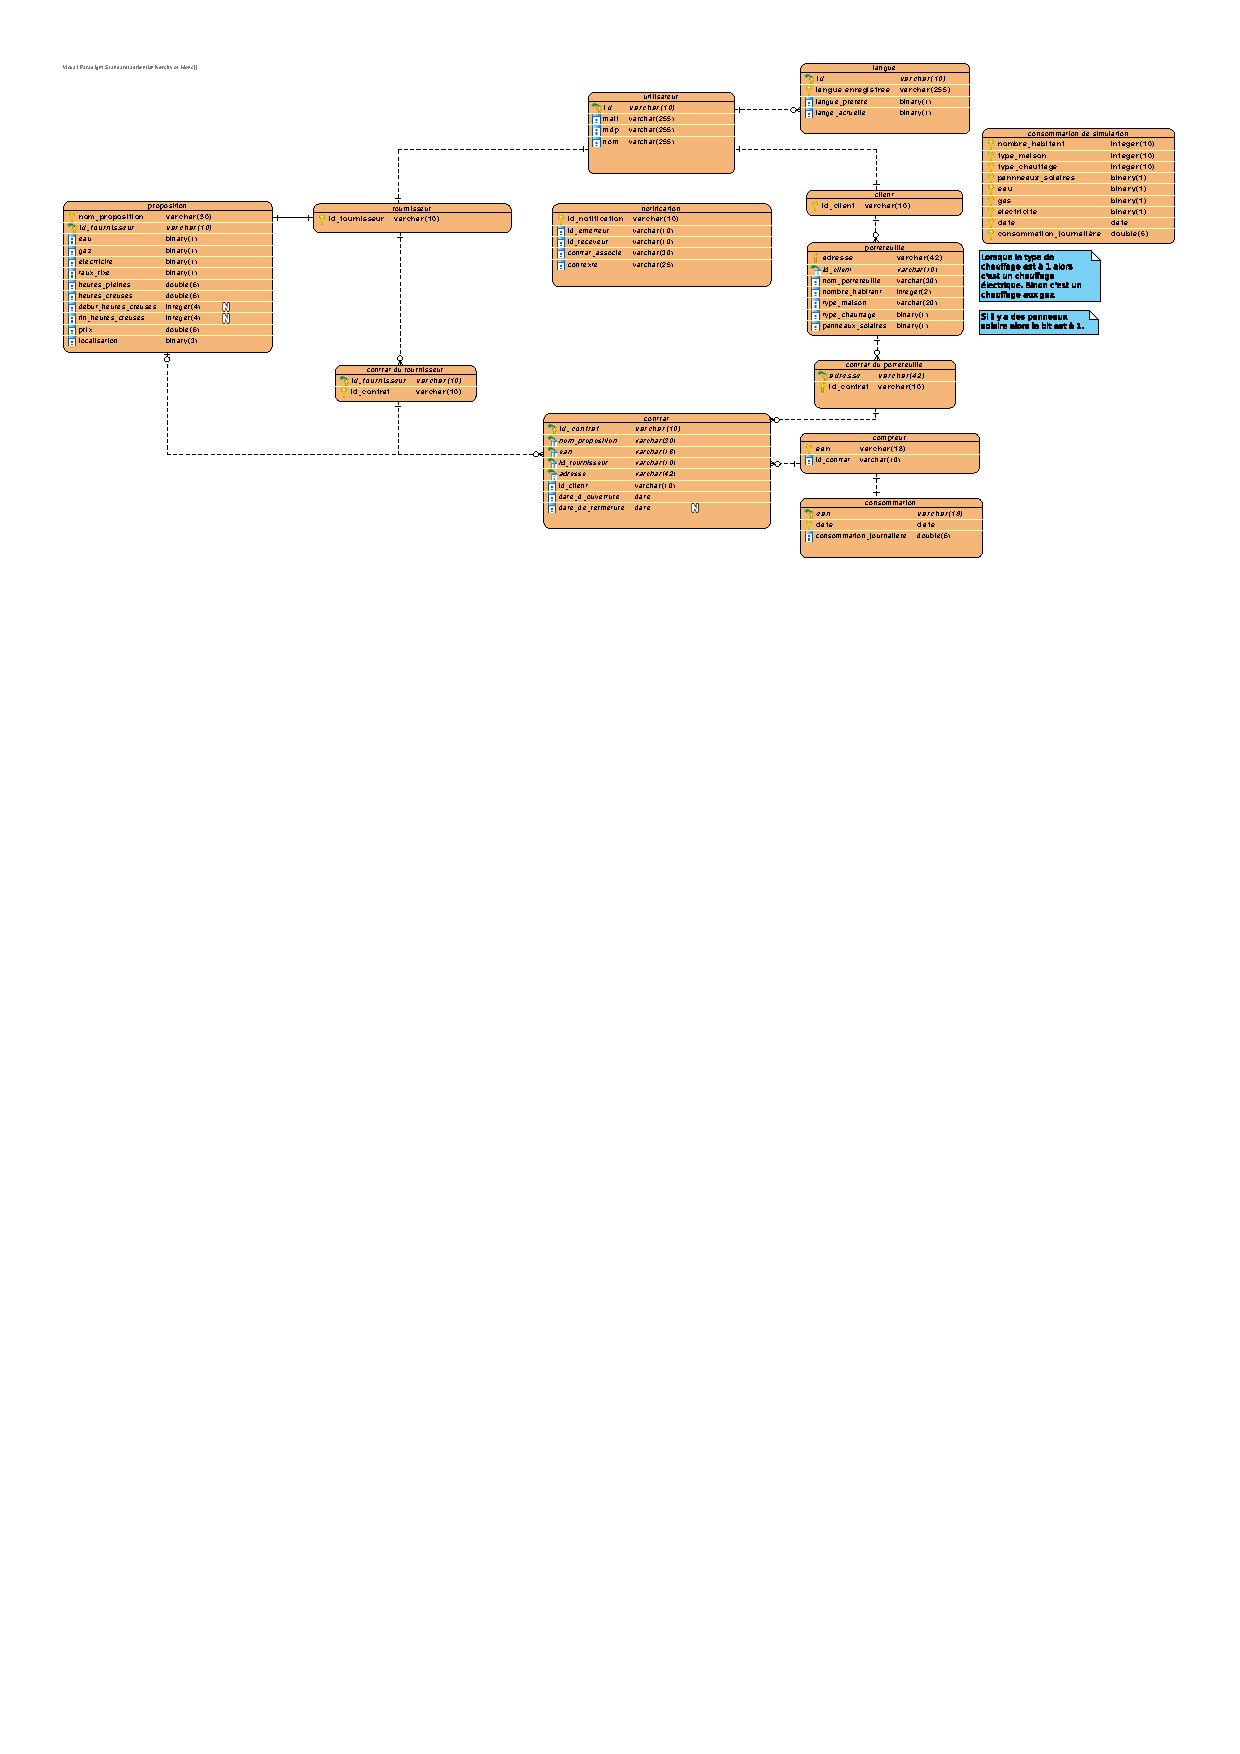
\includepdf[pages=-]{extension_adrien/Bdd/img/bdd.pdf}

\subsection{API}

\subsubsection{Introduction}

\begin{flushleft}
Dans cette partie, je vais vous expliquer les ajouts apportés à l'API de la base du projet. 
\end{flushleft}
\begin{flushleft}
Notez que les ajouts se trouvent dans ClientApi de ce package étant donné que cette extension ne concerne que les clients.
\end{flushleft}

\subsubsection{ClientApi}

\begin{flushleft}
Vous pouvez remarquer l'ajout des méthodes suivantes afin de faire la passerelle entre le front-end et la base de données.
\end{flushleft}

\begin{enumerate}
\item \textbf{getAllInvitedWallets} :\newline
Cette méthode permet d'appeler la méthode de "WalletManager" expliquée précédemment dans le but d'obtenir les portefeuilles "invités" avec la permission liée. 
\item \textbf{deleteInvitedClient} :\newline
Cette méthode permet d'appeler la méthode de "InvitedClientManager" afin de supprimer un invité. 
\item \textbf{changePermission} :\newline
Cette méthode permet d'appeler la méthode de "InvitedClientManager" afin de changer la permission d'un invité. 
\item \textbf{getAllInvitation} :\newline
Cette méthode permet d'appeler la méthode de "InvitationManager" dans le but d'obtenir toutes les invitations et refus ou acceptations de ces dernières. 
\item \textbf{proposeInvitation} :\newline
Cette méthode permet d'appeler la méthode de "InvitationManager" afin d'envoyer une invitation à un autre client pour espérer l'ajouter à la liste des invités. 
Cette méthode renvoie un code 500 si les conditions expliquées précédemment ne sont pas remplies.
\item \textbf{acceptInvitation} :\newline
Cette méthode permet d'appeler la méthode de "InvitationManager" afin d'accepter une invitation. 
Cette méthode renvoie aussi un code 500 si les conditions expliquées précédemment ne sont pas remplies.
\item \textbf{refuseInvitation} :\newline
Cette méthode permet d'appeler la méthode de "InvitationManager" afin de refuser une invitation. 
\item \textbf{deleteInvitation} :\newline
Cette méthode permet d'appeler la méthode de "InvitationManager" afin de supprimer une invitation. 
Cette dernière est également utile pour le front-end pour les invitations à marquer comme lues.
\end{enumerate}

\subsection{Front-end}

\subsubsection{Introduction}

\begin{flushleft}
Dans cette partie, je vais vous expliquer les modifications et ajouts apportés au front-end de la base du projet. 
\end{flushleft}

\begin{flushleft}
Vous pouvez constater l'ajout de quatres fichiers :
\end{flushleft}

\begin{enumerate}
\item \textbf{AddInvited}\newline
\item \textbf{ChangePermissions}\newline
\item \textbf{InvitationMessage}\newline
\item \textbf{InvitedWallet}\newline
\end{enumerate}

\subsubsection{AddInvited}

\begin{flushleft}
Cette page permet à un client d'ajouter un invité en saisissant l'identifiant de l'invité et en sélectionnant la permission qu'il souhaite lui accorder.
Cette manière de procéder semblait plus intuitive pour l'utilisateur, il suffit que la personne que ce dernier souhaite inviter aille dans ses paramètres pour voir son identifiant et ainsi lui donner.
\end{flushleft}

\subsubsection{ChangePermissions}

\begin{flushleft}
Cette page permet simplement de changer la permission d'un invité.
\end{flushleft}

\subsubsection{InvitationMessage}

\begin{flushleft}
Cette page répertorie toutes les demandes d'invitations et permet de les accepter ou refuser et de voir les demandes qui leur ont été refusées ou acceptées.
\end{flushleft}

\subsubsection{InvitedWallet}

\begin{flushleft}
Cette page permet comme expliqué précédemment de récupérer tous les portefeuilles où le client est invité ainsi que la permission correspondante.
\end{flushleft}
\begin{flushleft}
Notez que cette fois, lorsqu'on se dirige vers "walletFull", les permissions sont encodées dans le sessionStorage.
\end{flushleft}

\subsubsection{WalletFull et consumptionPage}

\begin{flushleft}
Ces deux pages reposent sur le même principe, je récupère la permission associée et grâce aux directives de condition, j'affiche les possibilités pour le client en fonction qu'il soit propriétaire ou s'il est invité en lecture ou lecture et écriture.
\end{flushleft}

\subsubsection{Modules importés}
\begin{enumerate}[-]
\item \textbf{jwt-decode} :\newline
Ce module est importé afin d'obtenir l'identifiant de l'utilisateur.
\end{enumerate}
\subsection{Conclusion}
\begin{flushleft}
Le développement de ce projet nous a permis d'acquérir de l'expérience concernant le fonctionnement d'un site comprenant une API et une base de données.
\end{flushleft}
\begin{flushleft}
Ce projet nous a beaucoup appris et nous a permis de mettre en pratique plus concrètement certaines notions\footnote{Le readme contient la documentation manipulée.}.
\end{flushleft}
\subsection{Readme}
\begin{flushleft}
Les tests unitaires relatifs à la partie backend fonctionnent parfaitement dans l'IDLE intellij. Malheureusement, il semble avoir un problème quand on tente d'effectuer \texttt{gradle test} dans le terminal. Ceci viendrait d'un problème d'accès à la base de données. Il a été tenté par différents moyens de résoudre le problème sans succès. De ce fait, les preuves de réussites des tests ont été déposé dans l'archive. 
\end{flushleft}


\section{Introduction: 1.6.4: Analyse statistique de la consommation énergétique}

\begin{flushleft}
Le but de cette extension est surtout de permettre au client de comparer ces données de consommation avec d'autres. Plusieurs possibilités seront proposées.
\end{flushleft}

\begin{flushleft}
D'abord, l'application pourra calculer des statistiques par rapport aux données du client. Ce dernier pourra choisir un intervalle de temps et en connaître les statistiques, en autre la moyenne, l'écart type, la médiane, les quartiles, l'écart interquartile ainsi que le minimum et le maximum. Le client pourra ensuite comparer toutes ces données avec les données de consommations qu'il souhaite.
\end{flushleft}

\begin{flushleft}
Ensuite, le client pourra comparer ses données en fonction de la date. En effet, il aura l'occasion d'afficher un deuxième tableau ou graphique et de choisir un autre intervalle de temps. Ainsi, il pourra par exemple regarder la différence de statistique entre sa consommation en hiver et en été.
\end{flushleft}

\begin{flushleft}
Finalement, il aura également l'occasion de comparer ses données de consommations avec les données d'autres clients ayant les mêmes caractéristiques (en pratique, ces données seront en réalité une simulation et non les données d'autres utilisateurs).
\end{flushleft}

\begin{flushleft}
Notez que cette extension implique une autre fonctionnalité. En effet, l'application surveillera chaque donnée de consommation introduite pour prévenir le client si une valeur est anormalement élevée. Un mail sera donc tout simplement envoyé pour expliquer que la donnée entrée est étrange. Le client pourra donc agir en conséquence.
\end{flushleft}

\subsection{Bdd}

\begin{flushleft}
Au niveau de la base de données, j'ai besoin dans un premier temps de stocker plus d'informations sur l'habitation des clients, c'est-à-dire dans la table \textbf{portefeuille}. Notamment le nombre de personnes habitant dans cette dernière, le type de maison, le type de chauffage et finalement s'il y a une présence de panneaux solaires.
\end{flushleft}

\begin{flushleft}
Dans un second temps, j'ai stocké les données de consommations qui serviront de comparaison. Pour cela, une nouvelle table a été crée, à savoir \textbf{consommation de simulation}. Nous devons donc y retrouver des données de consommations, un type d'énergie et une date mais il faut aussi pouvoir les distinguer en fonction des caractéristiques de la maison, c'est pourquoi nous y retrouvons également les mêmes types de données que dans la table portefeuille. C'est-à-dire le nombre d'habitants, le type de maison, le type de chauffage et s'il y a des panneaux solaires.
\end{flushleft}

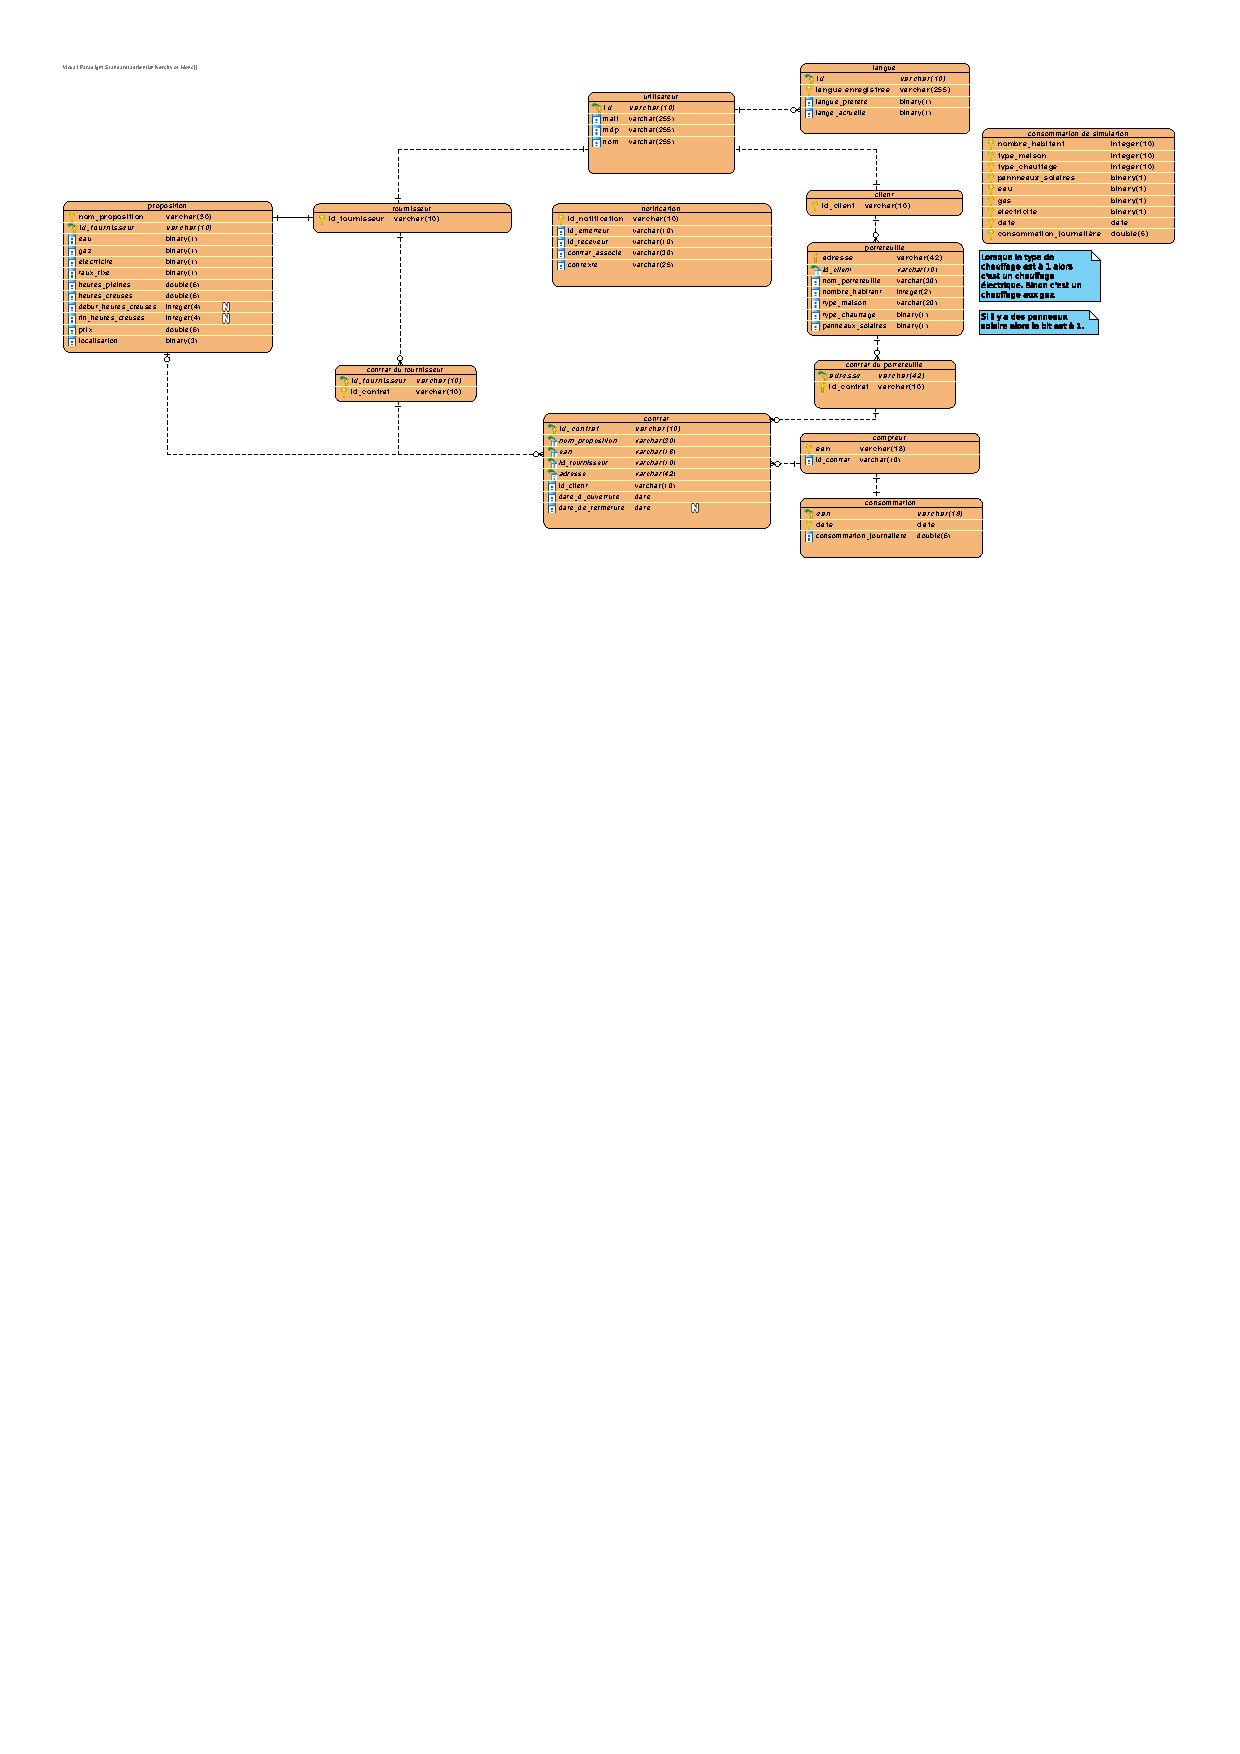
\includepdf[pages=-]{extension_adrien/Bdd/img/bdd.pdf}

\subsection{API}

\subsubsection{Introduction}

\begin{flushleft}
Dans cette partie, je vais vous expliquer les ajouts apportés à l'API de la base du projet. 
\end{flushleft}
\begin{flushleft}
Notez que les ajouts se trouvent dans ClientApi de ce package étant donné que cette extension ne concerne que les clients.
\end{flushleft}

\subsubsection{ClientApi}

\begin{flushleft}
Vous pouvez remarquer l'ajout des méthodes suivantes afin de faire la passerelle entre le front-end et la base de données.
\end{flushleft}

\begin{enumerate}
\item \textbf{getAllInvitedWallets} :\newline
Cette méthode permet d'appeler la méthode de "WalletManager" expliquée précédemment dans le but d'obtenir les portefeuilles "invités" avec la permission liée. 
\item \textbf{deleteInvitedClient} :\newline
Cette méthode permet d'appeler la méthode de "InvitedClientManager" afin de supprimer un invité. 
\item \textbf{changePermission} :\newline
Cette méthode permet d'appeler la méthode de "InvitedClientManager" afin de changer la permission d'un invité. 
\item \textbf{getAllInvitation} :\newline
Cette méthode permet d'appeler la méthode de "InvitationManager" dans le but d'obtenir toutes les invitations et refus ou acceptations de ces dernières. 
\item \textbf{proposeInvitation} :\newline
Cette méthode permet d'appeler la méthode de "InvitationManager" afin d'envoyer une invitation à un autre client pour espérer l'ajouter à la liste des invités. 
Cette méthode renvoie un code 500 si les conditions expliquées précédemment ne sont pas remplies.
\item \textbf{acceptInvitation} :\newline
Cette méthode permet d'appeler la méthode de "InvitationManager" afin d'accepter une invitation. 
Cette méthode renvoie aussi un code 500 si les conditions expliquées précédemment ne sont pas remplies.
\item \textbf{refuseInvitation} :\newline
Cette méthode permet d'appeler la méthode de "InvitationManager" afin de refuser une invitation. 
\item \textbf{deleteInvitation} :\newline
Cette méthode permet d'appeler la méthode de "InvitationManager" afin de supprimer une invitation. 
Cette dernière est également utile pour le front-end pour les invitations à marquer comme lues.
\end{enumerate}

\subsection{Front-end}

\subsubsection{Introduction}

\begin{flushleft}
Dans cette partie, je vais vous expliquer les modifications et ajouts apportés au front-end de la base du projet. 
\end{flushleft}

\begin{flushleft}
Vous pouvez constater l'ajout de quatres fichiers :
\end{flushleft}

\begin{enumerate}
\item \textbf{AddInvited}\newline
\item \textbf{ChangePermissions}\newline
\item \textbf{InvitationMessage}\newline
\item \textbf{InvitedWallet}\newline
\end{enumerate}

\subsubsection{AddInvited}

\begin{flushleft}
Cette page permet à un client d'ajouter un invité en saisissant l'identifiant de l'invité et en sélectionnant la permission qu'il souhaite lui accorder.
Cette manière de procéder semblait plus intuitive pour l'utilisateur, il suffit que la personne que ce dernier souhaite inviter aille dans ses paramètres pour voir son identifiant et ainsi lui donner.
\end{flushleft}

\subsubsection{ChangePermissions}

\begin{flushleft}
Cette page permet simplement de changer la permission d'un invité.
\end{flushleft}

\subsubsection{InvitationMessage}

\begin{flushleft}
Cette page répertorie toutes les demandes d'invitations et permet de les accepter ou refuser et de voir les demandes qui leur ont été refusées ou acceptées.
\end{flushleft}

\subsubsection{InvitedWallet}

\begin{flushleft}
Cette page permet comme expliqué précédemment de récupérer tous les portefeuilles où le client est invité ainsi que la permission correspondante.
\end{flushleft}
\begin{flushleft}
Notez que cette fois, lorsqu'on se dirige vers "walletFull", les permissions sont encodées dans le sessionStorage.
\end{flushleft}

\subsubsection{WalletFull et consumptionPage}

\begin{flushleft}
Ces deux pages reposent sur le même principe, je récupère la permission associée et grâce aux directives de condition, j'affiche les possibilités pour le client en fonction qu'il soit propriétaire ou s'il est invité en lecture ou lecture et écriture.
\end{flushleft}

\subsubsection{Modules importés}
\begin{enumerate}[-]
\item \textbf{jwt-decode} :\newline
Ce module est importé afin d'obtenir l'identifiant de l'utilisateur.
\end{enumerate}
\subsection{Conclusion}
\begin{flushleft}
Le développement de ce projet nous a permis d'acquérir de l'expérience concernant le fonctionnement d'un site comprenant une API et une base de données.
\end{flushleft}
\begin{flushleft}
Ce projet nous a beaucoup appris et nous a permis de mettre en pratique plus concrètement certaines notions\footnote{Le readme contient la documentation manipulée.}.
\end{flushleft}

\section{Introduction: 1.6.4: Analyse statistique de la consommation énergétique}

\begin{flushleft}
Le but de cette extension est surtout de permettre au client de comparer ces données de consommation avec d'autres. Plusieurs possibilités seront proposées.
\end{flushleft}

\begin{flushleft}
D'abord, l'application pourra calculer des statistiques par rapport aux données du client. Ce dernier pourra choisir un intervalle de temps et en connaître les statistiques, en autre la moyenne, l'écart type, la médiane, les quartiles, l'écart interquartile ainsi que le minimum et le maximum. Le client pourra ensuite comparer toutes ces données avec les données de consommations qu'il souhaite.
\end{flushleft}

\begin{flushleft}
Ensuite, le client pourra comparer ses données en fonction de la date. En effet, il aura l'occasion d'afficher un deuxième tableau ou graphique et de choisir un autre intervalle de temps. Ainsi, il pourra par exemple regarder la différence de statistique entre sa consommation en hiver et en été.
\end{flushleft}

\begin{flushleft}
Finalement, il aura également l'occasion de comparer ses données de consommations avec les données d'autres clients ayant les mêmes caractéristiques (en pratique, ces données seront en réalité une simulation et non les données d'autres utilisateurs).
\end{flushleft}

\begin{flushleft}
Notez que cette extension implique une autre fonctionnalité. En effet, l'application surveillera chaque donnée de consommation introduite pour prévenir le client si une valeur est anormalement élevée. Un mail sera donc tout simplement envoyé pour expliquer que la donnée entrée est étrange. Le client pourra donc agir en conséquence.
\end{flushleft}

\subsection{Bdd}

\begin{flushleft}
Au niveau de la base de données, j'ai besoin dans un premier temps de stocker plus d'informations sur l'habitation des clients, c'est-à-dire dans la table \textbf{portefeuille}. Notamment le nombre de personnes habitant dans cette dernière, le type de maison, le type de chauffage et finalement s'il y a une présence de panneaux solaires.
\end{flushleft}

\begin{flushleft}
Dans un second temps, j'ai stocké les données de consommations qui serviront de comparaison. Pour cela, une nouvelle table a été crée, à savoir \textbf{consommation de simulation}. Nous devons donc y retrouver des données de consommations, un type d'énergie et une date mais il faut aussi pouvoir les distinguer en fonction des caractéristiques de la maison, c'est pourquoi nous y retrouvons également les mêmes types de données que dans la table portefeuille. C'est-à-dire le nombre d'habitants, le type de maison, le type de chauffage et s'il y a des panneaux solaires.
\end{flushleft}

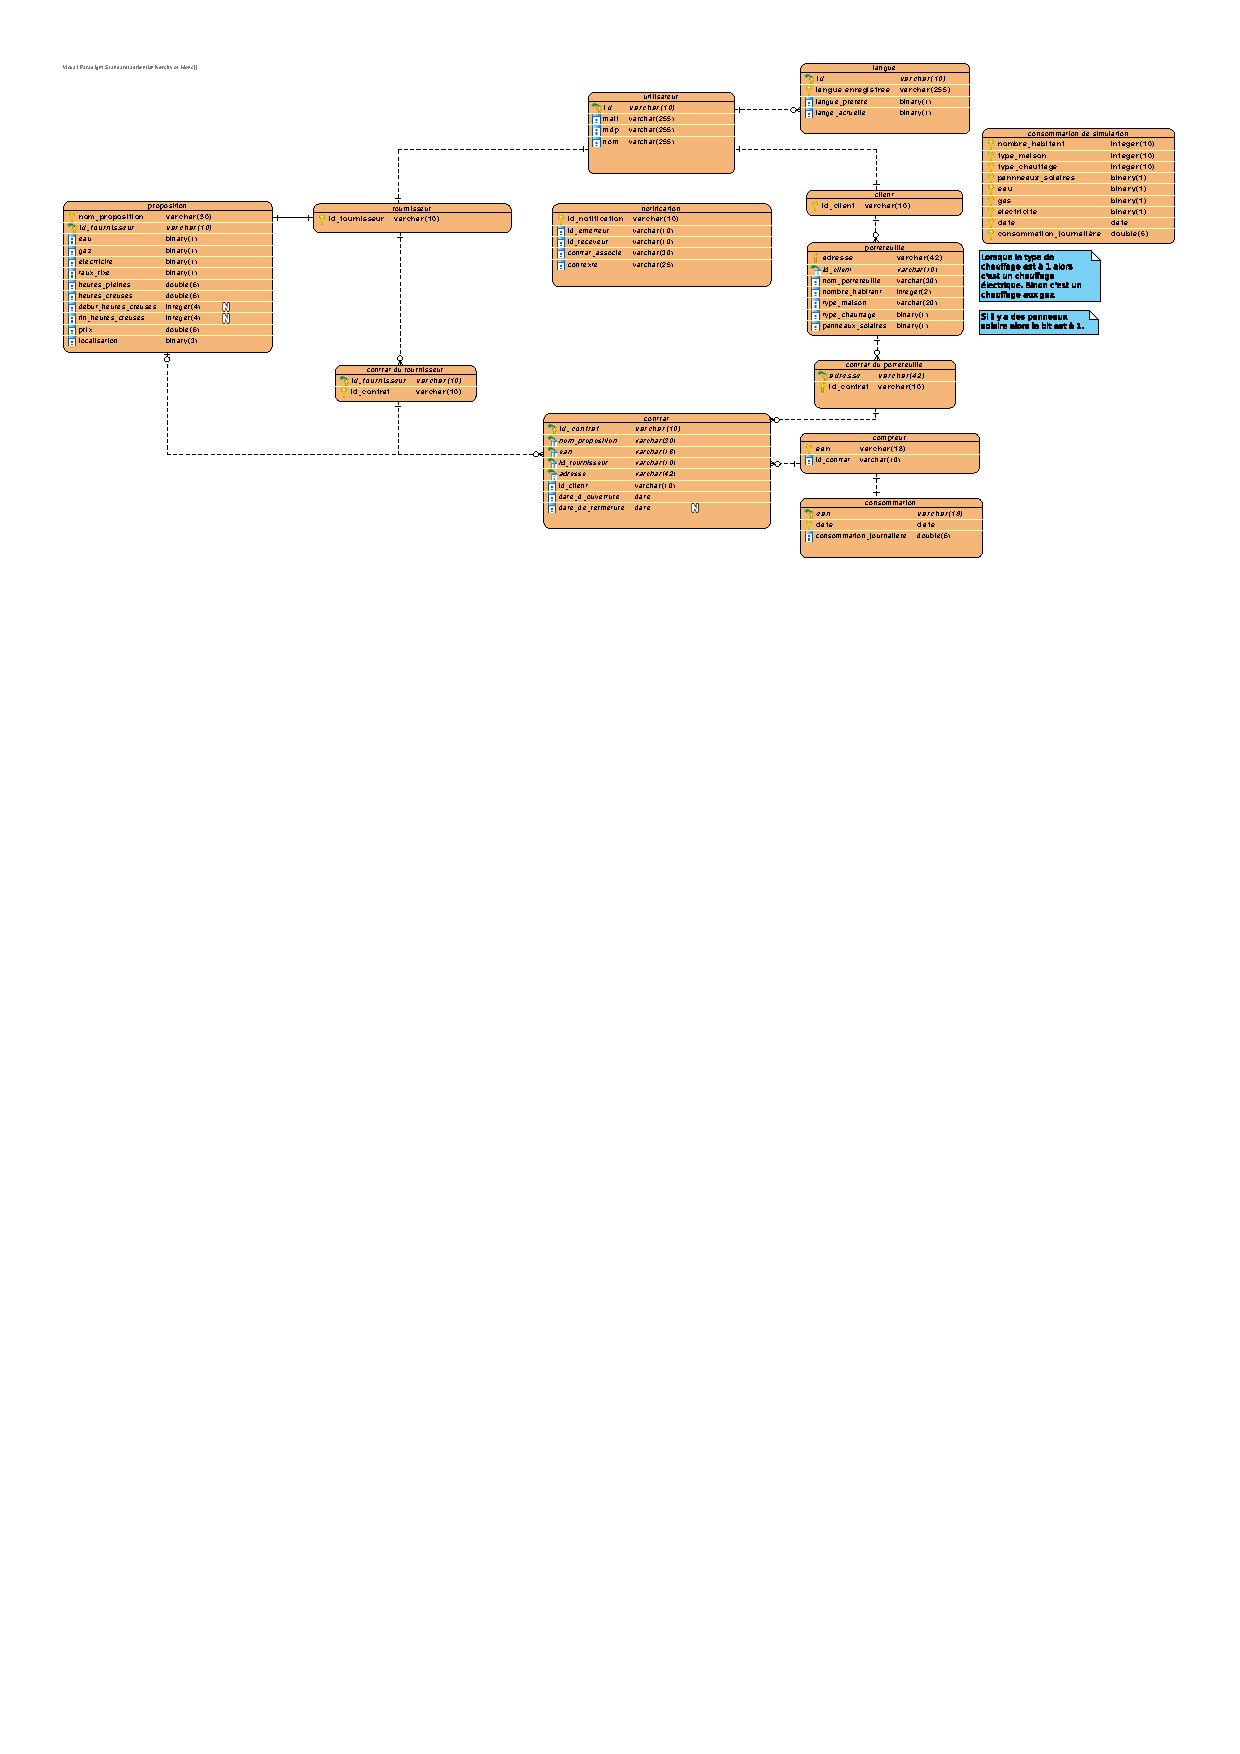
\includepdf[pages=-]{extension_adrien/Bdd/img/bdd.pdf}

\subsection{API}

\subsubsection{Introduction}

\begin{flushleft}
Dans cette partie, je vais vous expliquer les ajouts apportés à l'API de la base du projet. 
\end{flushleft}
\begin{flushleft}
Notez que les ajouts se trouvent dans ClientApi de ce package étant donné que cette extension ne concerne que les clients.
\end{flushleft}

\subsubsection{ClientApi}

\begin{flushleft}
Vous pouvez remarquer l'ajout des méthodes suivantes afin de faire la passerelle entre le front-end et la base de données.
\end{flushleft}

\begin{enumerate}
\item \textbf{getAllInvitedWallets} :\newline
Cette méthode permet d'appeler la méthode de "WalletManager" expliquée précédemment dans le but d'obtenir les portefeuilles "invités" avec la permission liée. 
\item \textbf{deleteInvitedClient} :\newline
Cette méthode permet d'appeler la méthode de "InvitedClientManager" afin de supprimer un invité. 
\item \textbf{changePermission} :\newline
Cette méthode permet d'appeler la méthode de "InvitedClientManager" afin de changer la permission d'un invité. 
\item \textbf{getAllInvitation} :\newline
Cette méthode permet d'appeler la méthode de "InvitationManager" dans le but d'obtenir toutes les invitations et refus ou acceptations de ces dernières. 
\item \textbf{proposeInvitation} :\newline
Cette méthode permet d'appeler la méthode de "InvitationManager" afin d'envoyer une invitation à un autre client pour espérer l'ajouter à la liste des invités. 
Cette méthode renvoie un code 500 si les conditions expliquées précédemment ne sont pas remplies.
\item \textbf{acceptInvitation} :\newline
Cette méthode permet d'appeler la méthode de "InvitationManager" afin d'accepter une invitation. 
Cette méthode renvoie aussi un code 500 si les conditions expliquées précédemment ne sont pas remplies.
\item \textbf{refuseInvitation} :\newline
Cette méthode permet d'appeler la méthode de "InvitationManager" afin de refuser une invitation. 
\item \textbf{deleteInvitation} :\newline
Cette méthode permet d'appeler la méthode de "InvitationManager" afin de supprimer une invitation. 
Cette dernière est également utile pour le front-end pour les invitations à marquer comme lues.
\end{enumerate}

\subsection{Front-end}

\subsubsection{Introduction}

\begin{flushleft}
Dans cette partie, je vais vous expliquer les modifications et ajouts apportés au front-end de la base du projet. 
\end{flushleft}

\begin{flushleft}
Vous pouvez constater l'ajout de quatres fichiers :
\end{flushleft}

\begin{enumerate}
\item \textbf{AddInvited}\newline
\item \textbf{ChangePermissions}\newline
\item \textbf{InvitationMessage}\newline
\item \textbf{InvitedWallet}\newline
\end{enumerate}

\subsubsection{AddInvited}

\begin{flushleft}
Cette page permet à un client d'ajouter un invité en saisissant l'identifiant de l'invité et en sélectionnant la permission qu'il souhaite lui accorder.
Cette manière de procéder semblait plus intuitive pour l'utilisateur, il suffit que la personne que ce dernier souhaite inviter aille dans ses paramètres pour voir son identifiant et ainsi lui donner.
\end{flushleft}

\subsubsection{ChangePermissions}

\begin{flushleft}
Cette page permet simplement de changer la permission d'un invité.
\end{flushleft}

\subsubsection{InvitationMessage}

\begin{flushleft}
Cette page répertorie toutes les demandes d'invitations et permet de les accepter ou refuser et de voir les demandes qui leur ont été refusées ou acceptées.
\end{flushleft}

\subsubsection{InvitedWallet}

\begin{flushleft}
Cette page permet comme expliqué précédemment de récupérer tous les portefeuilles où le client est invité ainsi que la permission correspondante.
\end{flushleft}
\begin{flushleft}
Notez que cette fois, lorsqu'on se dirige vers "walletFull", les permissions sont encodées dans le sessionStorage.
\end{flushleft}

\subsubsection{WalletFull et consumptionPage}

\begin{flushleft}
Ces deux pages reposent sur le même principe, je récupère la permission associée et grâce aux directives de condition, j'affiche les possibilités pour le client en fonction qu'il soit propriétaire ou s'il est invité en lecture ou lecture et écriture.
\end{flushleft}

\subsubsection{Modules importés}
\begin{enumerate}[-]
\item \textbf{jwt-decode} :\newline
Ce module est importé afin d'obtenir l'identifiant de l'utilisateur.
\end{enumerate}
\subsection{Conclusion}
\begin{flushleft}
Le développement de ce projet nous a permis d'acquérir de l'expérience concernant le fonctionnement d'un site comprenant une API et une base de données.
\end{flushleft}
\begin{flushleft}
Ce projet nous a beaucoup appris et nous a permis de mettre en pratique plus concrètement certaines notions\footnote{Le readme contient la documentation manipulée.}.
\end{flushleft}

\section{Extension 1.6.7 : Facturation et paiement d'accomptes}
\subsection{Introduction}
\begin{flushleft}
Lors de l'implémentation d'un fonctionnement de facturation, quelques modifications ont eu lieu par rapport à la phase d'analyse fait au premier quadrimestre. En effet, je ne m'étais pas rendu compte de la difficulté à implémenter cette fonctionnalité
\end{flushleft}


\subsection{Choix technologiques}
\begin{flushleft}
Tout d'abord, le language du language s'est porté sur le \textbf{java}. En dépis du fait qu'apprendre le Kotlin aurait été quelque chose d'extrèmement instructif, il aurait été impossible de fournir une application android.  
\end{flushleft}
\begin{flushleft}
    Ensuite, pour ce qui est de l'envoi/réception de requête. Il a été choisi de prendre le framework \textbf{retrofit}. Ce framework possède de multiples avantages tels que : apprentissage facile, dé/sérialisation automatique des objets, "type-safe", supporte plusieurs clients HTTP et il est extensible et customisable. En somme, il est très puissant.
\end{flushleft}
 \begin{flushleft}
     De plus, un design pattern d'architecture a été pris pour rendre le code le plus compréhensible possible. Celui-ci est le \textbf{Model-View-ViewModel} (MVVM). Celui-ci sépare la partie graphique, donnée et logique de l'application. Ceci nous permet d'avoir un code qui peut être facilement extensible.
 \end{flushleft}
 \begin{flushleft}
     Pour générer l'icone de l'application, un site web a été utilisé : \url{https://romannurik.github.io/AndroidAssetStudio/icons-launcher.html#foreground.type=clipart&foreground.clipart=android&foreground.space.trim=1&foreground.space.pad=0.25&foreColor=rgba(96%2C%20125%2C%20139%2C%200)&backColor=rgb(68%2C%20138%2C%20255)&crop=0&backgroundShape=circle&effects=none&name=ic_launcher}
 \end{flushleft}
 \begin{flushleft}
     Bien évidemment, le format du code de l'application est adapté à une app android.
 \end{flushleft}
\subsection{Difficultés rencontrées}
\begin{flushleft}
La raison principale du peu de contenu produit a été évidemment le temps. En effet, l'extension a commencé à être produite une semaine avant la remise de celle-ci. Bien qu'il aurait été possible d'y consacrer la majeure partie de la journée, la santée et l'union des cours priment.
\end{flushleft}
\begin{flushleft}
Ensuite, le fait de programmer en android n'est pas du tout une tâche aisée. Même si le java était déjà acquis depuis bien longtemps, de nouveaux aspects tels que les layouts, framework android, retrofit... se sont introduits dans le developpement nécéssitant de consacrer son temps à énormément de documentation. De plus, l'arborescence d'un projet android est très disparate.
\end{flushleft}
\begin{flushleft}
Enfin, même si l'extension compte pour 40\% de la note. Il faut avoir une base solide prête à toute épreuve. C'est pourquoi il a été choisi de se concentrer plus sur la base que l'extension.
\end{flushleft}
\subsection{Ressentis}
\begin{flushleft}
Quand j'ai commencé cette extension, je me suis dis : pourquoi ?. Pourquoi avoir pris cette extension ? Honnêtement, je ne sais pas. Je voulais certainement tester quelque chose de nouveau et c'est chose faite. En effet, J'ai appris plein de choses et il me reste tellement à découvrir ! En plus de cela, J'ai adoré. Ca faisait longtemps que je n'avais jamais autant aimé programmer(depuis le cours de projet d'info en BAC1) et de voir le résultat ! Ce fut une expérience très courte (une semaine et demi) mais très enrichissante et passionante.  
\end{flushleft}


\end{document}
